\setcounter{chapter}{1} 
\chapter{Theoretical Background} \label{ch:theoretical_back}
% Parametrization (atmospheric modeling), a method of approximating complex processes.
In this chapter I will present motivation, necessary theoretical background and practical implications to understand thee need for new predictions of cloud cover/cloud amount. Investigating a data driven approach for parameterization of clouds. Developing new tools for approximating the complex process of cloud formation. Hopefully this will contribute to the understanding of the physical process which is cloud formation. The data used in this project is a mixture of satellite retrievals and reanalysis data. No ancillary information is provided. See sections \ref{sec:era5} to \ref{sec:meteosat} for more detailed descriptions. 
\\ \\
The numerical methods used in this thesis are described in section \ref{sec:comp_met}. All the code is available on GitHub in the project repository named MS on \href{https://github.com/hannasv/MS}{https://github.com/hannasv/MS}. At this repository you will find everything you need to perform this experiment yourself. Descriptions for downloading data and retrieving the correct licences. 
\\ \\ 
There is project environment ready for installation, called \textit{sciclouds}. This is a conda envionment, the yaml-file lists the python packages and their versions used for running this code. Notebooks for conducting the experiments. Supplementary material for remapping satellite data and land-sea masks are available in a supplementary repository called \textit{MS-suppl} \href{https://github.com/hannasv/MS-suppl}{https://github.com/hannasv/MS-suppl}.

%\subsection{Cloud feedbacks from convection and fronts} %Cloud, circulation and climate sensitivity article.
\section{Parameterizations of clouds} \label{sec:param_clouds}
Parametrizations are a tool used in climate models to include the effect of subgridscale prosesses. This is done for several processes \textbf{give examples}. This thesis is only conserned with parametrizaions of cloud cover. The simplest form of cloud scheme is binary. Either the eintire pixel is covered by clouds or there is no clouds present. This is implemented as follows, if $RH > 100 \rightarrow CLA = 1$ else $CLA = 0$.
Sub gridscale variability in humidity is necesary to achive fractional cloud cover. This can be combined with a sub gridscale of temperature. Over the years reaserchers have tried to draw the distrubutions of these variables from observations and implement them into models. Vitualy all probability density functions, PDF's have been used to model either cloud cover or its dependant variables humidity, temperature and so on. They have not been sucesfull in finding a adaquate repreentation of cloud cover using this approach. \textbf{(siter Tomkins summary)}
\\ \\
Cloud cover is usually a combination of several parametrizations. Its common to have seperate schemes for ice-, liquid clouds and convections.
\textbf{Read more Tomkins}
\\ \\ 
%What is necessary to understand why clouds are Parameterisations. Cite that all climate models are wrong but some are useful.
\subsection{Parametrizations of clouds - Climate models} \label{sec:params_climate_models}
Climate models are an important tool for studying the effects of emissions/forcing on future climates. The \acrfull{ipcc} provide assessments report every ~10th year or so, providing a state of the art status update on the current knowledge of climate change. Since the previos assesment report there has been three spesial report A, B and C. 
\textbf{Les special report.} The previous report published was Assesment report 5, AR5 in 2013 and the next report is scheduled to be published in 2021. 
The ensamble of climate models included in AR5 is \acrfull{cmip5}. 
\acrshort{cmip6} are now being evaluated, thus there is less published literature. Even though its a bit old, we will mostly focus on the results in AR5. \textbf{Plus the findings in the special reports.}
\\ \\
% As mentioned before cloud feedbacks contribute with the largest uncertainty when computing the climate sensitivity. 
In resent years a lot of effort have been invested in improving the parametrizations of subgridscale processes. Among these clouds contribute with the largest uncertainty, approximately three times as large as other process i.e. relative humidity-lapse rate feedback (these processes shoukd not be viewed in isolation). The contributions of the clouds to the short wave component in the radiative budget is the main contributor to the uncertainty. Short wave cloud feedback. \textit{To this day neither observastions of global climate models, GCM's provide clear eveidence or contradict the low level clouds feedback}. There is no accepted basis to refuse a GSM \textit{a priori} \textbf{this increases the muli-model mean spead in climate sensitivity}. Missing representations of clouds microphysical processes related to opacity or cirrus (high altitude, composed of ice) clouds.
\\ \\
The computational cost of generating these large ensambles are limiting factor. Simplyfied models in terms of resolution and/ or complexity is common/often necesarry. 
\\ \\ 
Using idealised experiments they give model spread in \acrfull{ecs}. This describes the \textit{equilibrium change in global and annual mean surface temperature after doubling the $CO_2$ conditions from preindustrial times.}
For \acrshort{cmip5} the \acrshort{ecs} is $2.1^oC$ to $4.7^oC$.The is \textit{very high confidence} that clouds are the primary factor attributing to the wide range. This is not a very big improvement from Hansen et. al. 1984 first estimate of climate sensitivity which was the range $2.0^oC$ to $5.0^oC$. \textbf{explain idealised experiments.} Hansen et. al. ran their experiments using a coarse resolution of $8^o \times 10^o$ grid box (lat $\times$ lon) and a doubling of the $CO_2$ concentrations from 315ppm to 630ppm. The \acrshort{cmip5} \textbf{What more where you thinking here..?}

\subsection{ERA5} \label{sec:param_ERA5}
ERA5 is produced used IFS cycle 4lr2. This has a new cloud scheme or hydrological cycle. \textbf{Artikkelen forteller om oppdateringer fra sist era-interim produksjon ikke alt som finnes. Bedre å skrive denne etter du har skrevet i datasettet hvor }. Husk Tomkins jobber for ECMWF.


\subsection{Practical implications} \label{sec:practical_implications}
When conducting large machine learning project, such as this thesis its good to have a understanding of needs of the end product. What should it be used for? And how does it need to be implemented to be usefull in such a way. 
\textbf{Explain the strength and weaknesses of this approach for future implementations. Hva er tatt høyde for ved valg av data og lignende. Kan være nyttig for om folk reproduserer det og skal jobbe videre...}
%  when  using machine learning models as parametrization
One of the obvious downsides of using this data driven approach is the rigid resolution. It needs to be retrained in another resolution for it to be usefull in climate research. Climate models provide data in a wide range of different of spatiotemporal resolutions. Before implementing this model it would need to be retrained on the resolution of the climate model under development. Which includes both remapping the data set and retraining the model. This is a time consuming process involving finding a new set of hyperparameters suitable for the new resolution. Once trained machine learning models provide fast results even for complex parametrizations which is what makes them suitable. For global climate models you need to have access to training data all over the globe otherwise there is no point. This thesis is concerend with a region, in order to compute a proof of consept. Antoher issue is that most machine learning packages are in python programming languange while climate models are in \textbf{fortran 90/95 - dobbelsjekk}. \textbf{how to solve this}

\section{Data set and Methods}
\subsection{ERA5} \label{sec:era5}
ERA5 is the latest in the series of reanalysis produced by \acrfull{ecmwf}. Re-analysis is as close to observations as one can get coherent in space and time. Sometimes people forget that it is assimilated against observations not observations. Data assimilation takes in observations and tries to make a accurate estimate of the state of the system. This includes observations from ground based, ships, bouyes, airplanes and satellites. The analysis is produced in the operational system, making it available within five days of real time. ERA5 is based on the Integrated Forecasting System, IFS cycle 4lr2. The data is available in $0.25^o$ degree and hourly resolution. Its an important product in the continuous climate monitoring of the earth system. Since we are learning from data its important to mention that the all sky radiance's from \acrfull{msg} in the period 2003-2012 is included in the assimilation. This is the same satellite as I gather the cloud masks. From more information on how the cloud mask are computed please read section \ref{sec:meteosat}.
\\ \\ 
Reanalyses data is often mistakenly referred to as observations. The differences between them was the theme of a essay in \acrfull{bams}, 2015. They conclude with that they are not to different. Both involve inference (theory based calculations) and re-analysis relies on forecast and observations does not. This is not a significant difference as long as the forecast is sufficiently accurate. Its important to be aware of that the uncertainty of the reanalysis is less well known than for observations. This makes it harder to judge appropriate use of the reanalysis.  

\subsection{METEOSAT Second Generation - SEVRI} \label{sec:meteosat}
The highest resolved satellite retrivals come from geostationary meteorological weather satellites. Polar orbiting satellites usually provide daily resolution.\textbf{ (STUBENAU)}. There is also a wide range of viewing angles. Optical properties is always a function of viewing angle and frequency (Huang et. al. 2018).  
\\ \\
%The orbit of MODIS makes sure it has the exact same viewing angle every 16th day. 
The angle attributes to small differences in detected cloud mask. This becomes evident when the standby and operational satelite scan simultaneously. By default the stanby satelite is adjusted to fit the position of the operational. By taking the difference some small patterns becomes visible. This is not accounted for when using the data. 
\\ \\ 
The second generation satellite consist of METEOSAT 8 to 11. The MSG system provides a two satellite system. The operational satellite at a nadir point of $0^o$ latitude. 
\\ \\ 
Sometimes both satellites gather data at the same time. Then the standby-satellite grid is rectified to a a grid of the operational one (Personal correspondence with the help-desk). In these images it becomes evident that viewing angle affects the retrievals. When this duplication occurs, the operational satellite is chosen. The temporal resolution of 15min and the nadir pixel size is 3km (Taravat, 2015). The sensor SEVERI har 12 channels. One broadband visible channel, three solar channels (0.6, 0.8 and 1.6 $\mu m$) and 8 thermal infrared channels (3.9, 6.2, 7.3, 8.7, 9.7, 10.8, 12.0 and 13.4 $\mu m$). (Taravat, 2015 - should probably find the source online on EUMATSAT web pages).
\\ \\ 
\textbf{More practical implications}. This one has two partners covering the Indian and Pacific ocean. Together they give almost a global view, discarding the poles. This will be useful if this trail run is successful.  \textbf{programming language. how to best implement them in }
%You may calculate the difference of the measurements, e.g. for channels VIS0.6, IR3.9 and IR10.8 between the two satellites. This will give an estimate how large the measurements differ and as a consequence the products (e.g. cloud mask) will be different.\textbf{also personal corespondance.}

\subsection{EUMETSAT Cloud Mask} \label{sec:EUMETSAT_cloud_mask}
The EUMETSAT cloud mask, CLM relies on the fact that clouds are colder and more reflective than the surface. They also reclassify isolated pixel. The data is available on Earth Observation Portal on EUMETSATS web pages. CLM consist of four classes, zero - clear sky over ocean, one which is clear sky over land, 2 denotes cloudy and 3 is outer space/off earth disk/no data. These classes are derived from almost all channels except (X) \textbf{cite article 10 in Tavarat, 2015}.

The cloud mask is distributed in GRIB-format (no coordinates) and NC-format (coordinates). Due to spatial limitations (Since all files have the same coordinates) one NC-files is downloaded for the coordinates and the rest of the data has been downloaded in GRIB-format. Some retrievals are excluded because of high uncertainty in the measurements this creates gaps in the data set. 

%\subsection{MODIS - If you include comparisons to verify own sat elite computations.} \label{sec:modis}
%\textbf{Something on modis.}
% Please add the following required packages to your document preamble:
% \usepackage{multirow}

\subsection{Thoughts when choosing the data set of satellite images}
Choose the finest temporal resolution possible. The average lifetime of a cloud is an hour. Since this is a proof of study is seems reasonable to choose the finest resolution available. Here this is METEOSAT. 
\\ \\
In future work it would be interesting to asses how data driven parametrization compare to the existing parametrizaions available in the state of the art climate models. Here both the temporal and spatial resolution is a lot coarser. Other data sets could be considered. The masks in other data sets are computed based on more channels than in METEOSAT but the temporal resolution is a lot worse. 

\subsection{European Cloud Cover} \label{sec:ECC}
\textit{Add somewhere from personal correspondence the gaps are caused by: We regret to inform you that unfortunately we cannot process your orders 1368572 and 1368598. The data was corrupted prior archiving to tape and this data file cannot be recovered. }
For the purpose of this thesis a new data set was built. The clouds in ERA5 is models according to the descriptions in \ref{sec:param_ERA5} so I had to look elsewhere for a suitable \textit{true value} to regress the meteorological variables against. Keep in min the hourly temporal resolution and $0.25^o$ spatial resolution in ERA5. Most satellite products move in polar orbits and finer resolution than daily is rare. Vertically resolved data was also unnecessary. \textbf{cite Calipso and Modis}. This guided me in the direction of the satellites in geostationary orbit. The only geostationary satellite covering the east Atlantic is the 0 degree \acrfull{msg} satellite. With the high temporal resolution of 15min and a fixed grid is seemed like a reasonable choice. %This is beneficial when learning from data. 
Preserving the resolution available from ERA5, remapping the cloud mask to cloud fractions also know as cloud amount. \textit{\acrshort{ecc} comprises of five variables collected from two sources; ERA5 and EUMETSAT}The final product consist of the variables temperature, pressure, cloud amount, specific and relative humidity. Hourly data on a $0.25^o$ resolution in the period \textbf{put in first date} to \textbf{last date}. 
For this project the geographical domain has been restricted latitude $\in[30,50]$ and longitude $\in [-15, 25]$. This becomes 80x160 pixels for each time step. As always when working with observations, data is missing. Since the individual pixels are remapped to fractions by using the area weighted mean, NaN's are not a issue. For sometimes no cloud masks are available. Then the closest time step available within the previous and trailing 45 minutes are chosen. Other gaps are documented in \textbf{X}. 
\\ \\
The original data is described in table \ref{tab:dataset_summary} and the finished product is described in the \ref{tab:ecc}. The demanding process of remapping the mask to fraction is presented in section \ref{sec:remapping}
% more detailed description on what ERA5 is and how it is produced is described in section \ref{sec:era5}. 
% As table \ref{tab:variables} shows the data set comprises of five variables collected from two sources; ERA5 and EUMETSAT. Temperature, surface pressure, specific and relative humidity is collected from ERA5. More information about this is available in section \ref{sec:era5}.
Fractional cloud cover is computed from the cloud mask product retrieved by the second generations METEOSAT satellites. You can read more about this data in section \ref{sec:meteosat}. For simplicity we will refer to this dataset as European Cloud Cover Dataset, ECC from now on. 
\\ \\ 
%This includes METEOSAT 8, 9, 10 and 11.
The mapping from the curve-linear grid of the geostationary satellite to the uniform grid of era5 is quite technical and is described in section \ref{sec:regridding}. The cloud amount of a pixel is the sum of the area weighted cloud mask contributing to a cell.
\textbf{transponer tabellen!!!!}

\begin{table}[]
\begin{tabular}{|c|c|c|c|c|c|}
\hline
\textbf{Source}                & \multicolumn{1}{c|}{\textbf{Type}}               & \textbf{Variables}         & \textbf{Projection}                    & \textbf{Availability}          & \textbf{Licence}                                                                                                                   \\ \hline
\multirow{4}{*}{ERA5} & \multirow{2}{*}{Surface}                & 2m Temperature    & \multirow{4}{*}{Uniform grid} & \multirow{4}{*}{1979 - dd.} & \multirow{4}{*}{\begin{tabular}[c]{@{}c@{}}Need user on \\ Copernicus Data Store. \\ Available for everyone.\end{tabular}} \\
                      &                                         & Surface pressure  &                               &                             &                                                                                                                            \\
                      & \multirow{2}{*}{1000 hPa}               & Relative Humidity &                               &                             &                                                                                                                            \\
                      &                                         & Specific Humidity &                               &                             &                                                                                                                            \\ \hline
MSG                   & \multicolumn{1}{c|}{Satellite retrival} & Cloud Mask        & Curvelineaer grid             & 2004-dd.                    & \begin{tabular}[c]{@{}c@{}}Higher than 3hourly \\ resolution requires a \\ reaserchers liscence.\end{tabular}              \\ \hline
\end{tabular}
\caption{Data description on the data present in the dataset ECC (European Cloud Cover). \textbf{Add projection as a column, Availability for download and the period of data.} There is a lot of work in combining the two datasets and processing it.}
\label{tab:dataset_summary}
\end{table}

\begin{figure}[h]
    \centering
    \includegraphics[scale = 0.7]{Chapter2_Theory/images/Domain.png}
    \caption{Map showing the domain. The region cover southern Europe and northern Africa. The coordinate system is Plate Caree, which is the same as ECC. The image have been generated using the python package cartopy ref? \textbf{new figure with correct range and some vegetation or topography on  }}
    \label{fig:map}
\end{figure}

\begin{figure}[h]
    \centering
    \includegraphics[scale=0.11]{Chapter2_Theory/images/MET10_RGBNatColourEnhncd_FullResolution_20191123120000.jpg}    \caption{The view of the earth from \acrshort{msg}. The picture is dated noon on the 11 November 2019. \textbf{Cite EUMETSAT}. By studying the patterns it becomes evident that clouds are influenced by the circulations. }
    \label{fig:sat_view}
\end{figure}

%%%%%%%%%%%%%%%%%%%%%%%%%%%%%%%%%%%%%%%%%%%%%%%%%%%%
\subsubsection{Physical basis of variable decision} \label{sec:physical_basis}
The variables have been chosen based on availability, \textit{uncertainty/ quality} and their contribution to the physical processes. As mentioned in the introduction clouds require a aerosol and sufficient supersaturation.\textit{ However up-draft velocities and aerosols (especially type) is difficult to impossible to know?} \textbf{kilde?} I hypothesis that some of this information is present in temperature, humidifies and surface pressure in space and time and thus the cloud cover can be inferred patterns of these variables. Except for rural areas there is usually \acrshort{cnn} and/or \acrshort{inp} present. \textbf{lov å si kilde!}

\paragraph{Temperature}\mbox{}\\ % Need this line otherwise its 
The temperature is the two meter temperature produced by ERA5. For simplicity this will be referred to as temperature from now on. High temperature is related to convection. The air close to the surface gets heated, this reduces the density and starts the process of rising air masses. As the air rises it cools as a consequence of the work that has been done to the surrounding because of expansion. The temperature could also be a seasonal proxy. 

\paragraph{Humidity} \mbox{}\\
Both specific and relative humidity is included as features. Conditions where relative humidity exceeds 100\% are called supersaturated. Intuitively this should be a good predictor. However since the the clouds don't form at the surface its not clear if specific humidity is a better predictor. Specific humidity is the actual amount of vapour in the atmosphere in units of \textbf{kg/kg?}. \textit{Trude: Can I say that the rate of evaporation at the surface is proporsjonale to the humidity?} To some extent these variables are temperature dependant. Warm air can retain more vapour than cold air. Which is the main reason from precipitation. 
\\ \\
Let humidity be a collective term for both humidity's. The data is gathered from the model level closest to the surface. Which is at a height of 1000hPa. 
\\ \\ 
In order to form a cloud you need the air to exceed a saturation with respect to water or ice. This can with the presence of cloud condensation nuclei/ ice nuclei particles start the cloud formation processes.  On the other hand specific humidity is the actual amount of water vapour present in the atmosphere. 

\paragraph{Surface Pressure}\mbox{}\\ % ikke samme linjeavstand
Due to the earth geometry and the angle of rotation there is a energy surplus at the equator. Winds transport some of this heat pole ward. Geostrophic winds are the large scale balance between the Coriolis force and the pressure gradients. This wind flows parallel to the isobars, lines of constant pressure. Any factor that generates a pressure gradient can create disruptions in the wind pattern's. Topography for instance. For convenience surface pressure will be referred to as pressure in this thesis. \textbf{Don't think including the equation from geostrophic balance improved this section.}
%%%%%%%%%%%%%%%%%%%%%%%%%%%%%%%%%%%%%%%%%%%%%%%%%%%%%%%%%%%%%%%%%%

\subsubsection{Computing cloud fractions} \label{sec:remapping}
The cloud fractions in \acrshort{ecc} is the area weighted cloud masks from \acrshort{msg}. The masks in \acrshort{msg} referred to as clear (0) or cloudy (1).
If there is a NaN present, this pixel is simply excluded. Calculation wise this has the same affect as a clear pixel. \textbf{Should this be updated to remove the area of the cloudy pixel.} 
\\ \\
The METEOSAT cloud mask provided in NetCDF-format contains the coordinate information. Since the coordinate system is constant only one NetCDF files are downloaded.The surface area of a square on a sphere can be computed by solving the integral in \eqref{eq:sphere_integral}. This is the result in \eqref{eq:sphere_finish}. Since the netCDF-files only contain latitude and longitude informa

Before using this formula approximations of the extent of the cell needs to be made.
    
Calculating the area based on a curve-linear grid that only contain information about latitude and longitude involves some simplifications. From \eqref{eq:sphere_finish} 

, which can be rewritten into equation \eqref{eq:sphere_finish}. The latter one is used for implementations. Here R denotes the distance to earth centre, $\theta$ the latitude and $\phi$ the longitude. Approximation of $d\phi$ and $d\theta$ have been done based on the two-dimensional fields of latitude and longitude values according to equations \eqref{eq:app_lon} and  \eqref{eq:app_lat}.

%I have tried to keep these to a minimum and believe that they don't add more uncertainty. 
The visual comparison between raw satellite images and cloud amount seem to agree. The cloud fractional distribution also retain the same shape as ERA5 and MODIS 6.1 terra in the period from 2004 to 2018. 
\\ \\
\textbf{Update equation to use a upside down delta.}
\begin{equation} \label{eq:sphere_integral}
    A = -R^2\int_{ \theta - \delta \theta }^{\theta + \delta \theta} \int_{ \phi - \delta \phi }^{\phi + \delta \phi} cos\left( \theta' \right) d\phi' d\theta'
\end{equation} 

\begin{equation} \label{eq:sphere_finish}
    A \left( \theta, \phi, \delta \theta, \delta \phi   \right)= 2R^2 \left( sin\left( \theta + \delta \theta  \right) - sin\left(  \theta - \delta \theta  \right) \right) \delta \phi
\end{equation} 

The latitude and the extend of the pixel is terms in this equation. The extent of a pixel can also be interpreted as the \textbf{what.} The changes on longitude at a certain pixel is the the average distance to neighbouring points.

\begin{equation} \label{eq:app_lon}
    \delta \phi_{i,j} = \left| \frac{\phi_{i+1,j} - \phi_{i-1, j}}{4} \right|
\end{equation}

\begin{equation} \label{eq:app_lat}
    \delta \theta_{i,j} = \left| \frac{\theta_{i,j+1} - \theta_{i, j-1}}{4} \right|
\end{equation}

The latitude, longitude information is retrieved from the product of the satellite images. In order to keep the data storage to a minimum most files are download in grib-format. All satellite images from the 0 degree service are given with the same coordinates. This became evident from conversation with the help desk. 
\begin{figure}[h]
    \centering
    \includegraphics[scale = 0.6]{Chapter2_Theory/images/coordinates.png}
    \caption{Credit, https://tex.stackexchange.com/questions/159445/draw-in-cylindrical-and-spherical-coordinates}
    \label{fig:coords}
\end{figure}

The cloud cover will be referred to as cloud amount, fraction or simply the clouds.
%%%%%%%%%%%%%%%%%%%%%%%%%%%%%%%%%%%%%%%%%%%%%%%%%%%%%%%%%%%%%
\subsubsection{Licences and Downloading Data} \label{sec:downloading_data}
Scripts for downloading the ERA5 data used in this thesis is available in the project GitHub on \href{https://github.com/hannasv/MS/tree/metos/downloading{\_}RA}{https://github.com/hannasv/MS/tree/metos/downloading{\_}RA}. However you will need to create a CDS-user. I suggest you follow the instructions on ECMWF homepages on \textit{how to download ERA5}. 
There are no scripts available for downloading METEOSAT data this is done using satellite retrievals at EUMETSATs Earth Observation Portal. Its freely available in hourly resolution. Scientist can apply for increased resolution up to 15min. You choose the cloud mask product in grb-format. By running \textbf{X - legg inn filnavn} you can remap your own files.

%%%%%%%%%%%%%%%%%%%%%%%%%%%%%%%%%%%%%%%%%%%%%%%%%%%%%%%%%%%%%%%%%%
\subsubsection{summary}
In this thesis I want to test if its possible to make a parametrization on total cloud cover based on macro-scale variables like humidity, surface temperature and pressure. Move away from the subgridscale processes, by regressing historical observations against macro physical properties which affect clouds. The question remains: Is there be enough information in humidity, temperature and surface pressure to predict clouds in a time and space. 

\begin{enumerate}
    \item How representative is the training period we choose?
    \item politikk - machine learning velger personalisert reklame i forhold til valg.
    \item speech recognition (google speaker)
    \item spam filter 1990
    \item selv kjørende buss - aker brygge 
    \item manipulere video - at du får politikere / andre til å si ting de aldri har sagt
    \item face generation
    \item testing (in-sample error) and validiation (out of sample error) - generalization error 
    \item pipeline - transformations of cloud cover data. 
    \item predicting house prices is a typical regression task. Predicting if a person will default on its loan is another one. 
    \item clustering and classification as examples on mnist (overused dataset)
    \item Stuff on downloading data and installing the envionment can be called \textit{setting up your workspace -- > downloading data}
    \item Look at the correlation in the data. Pearson correlation? Someone else correlation?
    \item \textit{This plot reveals several things. First, the correlation is very strong. Second, ... }
    \item \textit{You will often gain good insight on the problem by examining }
    \item Ensamble methods in climate models and machine learning. It true that for both domains the model mean usually outperform the single model.
\end{enumerate}


\section{Machine learning} \label{sec:intro_machine_learning}
In this section I will explain the computational methods used for generating the numerical experiments conducted in this thesis. Starting with the the performance metrics used to evaluate the models. Followed by the auto regressive model and recurrent neural networks. For recurrent nets I will start by explaining the simple feed forward network building up to the more complex recurrent networks. This network is also known as convolution long short-term memory network. \textbf{Anatomy and architecture.} 
\\ \\
Machine learning is a part of our daily life. From self driving bussed in  your 

is a word on a lot of peoples tounge. It becoming more and more a part of our daily life from search engines to googles speakers responding to speech. There are lot of different types of machine learning, suitable for solving different tasks. Figure \ref{fig:machine_learning_categories} shows the types of machine learning and their subcategories. Supervised learning is the part of machine learning concerned with learning the relation between input data, x and labelled data y. Regression predict continuous values. Replicating a function. Classification is discrete, since it assigns a category to the input. Reinforcement learning is solves games, labyrinth and fluid mechanics \textbf{(Jean Rubalt)}. Unsupervised learning tries to detect patterns in unlabelled data. This includes contains clustering and dimensionality reduction. Unsupervised and reinforcement learning is out of the scope of this thesis and will not be further discusses.
%author : Hanna Svennevik
\begin{figure}[hp]
    \centering
    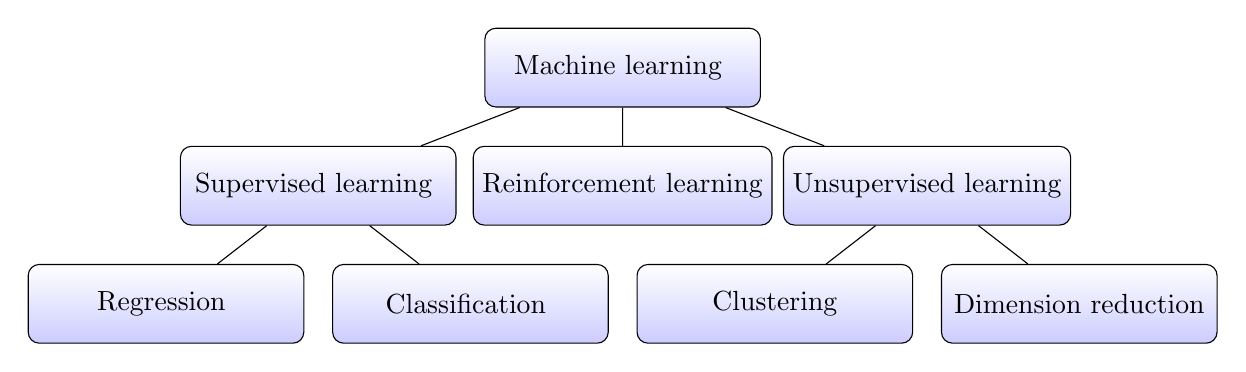
\begin{tikzpicture}[sibling distance=11em,
  every node/.style = {shape=rectangle, rounded corners,
    draw, align=center, 
    top color=white, bottom color=blue!20, minimum width=3.5cm, minimum height = 1.0cm}]]
  \node { Machine learning }
    child { node {  Supervised learning  } 
        child { node {  Regression   } }
        child { node {  Classification  } }
    }
    child {node {Reinforcement  learning}}
    child {node {Unsupervised learning}
           child { node {Clustering}}
           child { node {Dimension reduction}}};
\end{tikzpicture}
    \caption{Graph showing types of machine learning and their subcategories.}
    \label{fig:machine_learning_categories}
\end{figure}
There is a ongoing debate on what is intelligence. Traditionally a machine would be considered intelligent if it would beat a human at a given task. This has later been abandoned. The abilities a machine need to posses in order to beat a human in chess is completely different. A human needs X while the machine need Y. \textbf{kilde Chollet google} This will not be further discussed in this thesis since this is about task specific intelligence. Is it possible to train a network to gain sufficiently intelligent at the task of prediction European cloud cover?

\subsection{Supervised learning} \label{sec:supervised_learning}
Linear regression is the simplest form of supervised learning. Finding a suitable curve for a set of points. Working with real data, there is usually noise present in the dataset. In order to compensate for this we split the data into training and test (validation) sets. Overfitting becomes evident when you have a increase in the difference between the test- and training error. In non-mathematical terms, you have adjusted to much to the training data and where not able to find the general relation or "rules". See figure \ref{fig:linreg_overfitting}

\begin{figure}[hp]
    \centering
    \includegraphics{Chapter2_Theory/images/linear_regression.png}
    \caption{Fitting at different levels. The optimal fit is the most general one. This is applicable to many cases.}
    \label{fig:linreg_overfitting}
\end{figure}

\subsubsection{Autoregressive models} \label{sec:ARmodels}
The autoregressive model is a form of linear regression models where you allow a certain number of timesteps to be predictor variables. Equation \eqref{eq:AR-expression} describes how to make a prediction based on the optimal weighs, $\beta$. The expression for finding the optimal betas in a matrix form is given in equation \eqref{eq:AR-solution}. In the case for linear regression (using MSE- loss) there is only one solution to the optimal beta values. This makes it computationally very fast, as long as the matrix $X^TX$ is non-singular and thus its inverse exits. \textbf{Should i derive equation \eqref{eq:AR-solution}?}. For more complicated loss surfaces, there is no analytical solution. Gradient descent is a common algorithmn used to work around this. \textbf{write a section on gradient descent. Illustrert med mann som går ned fjellet og } 

\begin{equation} \label{eq:AR-expression}
    \hat{Y_n} = \hat{\beta_0} + \sum_{j=1}^p X_j\hat{\beta_j} + \sum_{i = 1}^{n_{ts}} Y_{n-i}\hat{\beta_{p+i}}
\end{equation}

\begin{equation} \label{eq:AR-solution}
    \hat{B} = \left( \textbf{X}^T\textbf{X} \right)^{-1}\textbf{X}\bar{y}
\end{equation}

\subsubsection{Transforming data} \label{sec:transforming_cloud_cover}
Since cloud cover fractions are in the range from zero to one, a common approach can be to transform the data so it includes values from the entire real axis $(-\infty, \infty)$. This is done using the inverse of the sigmoid function (see figure \ref{fig:sigmoid}).
% Exmale on sigmoid use this to include other plots you will use. 
\begin{figure}[hp]
    \centering
    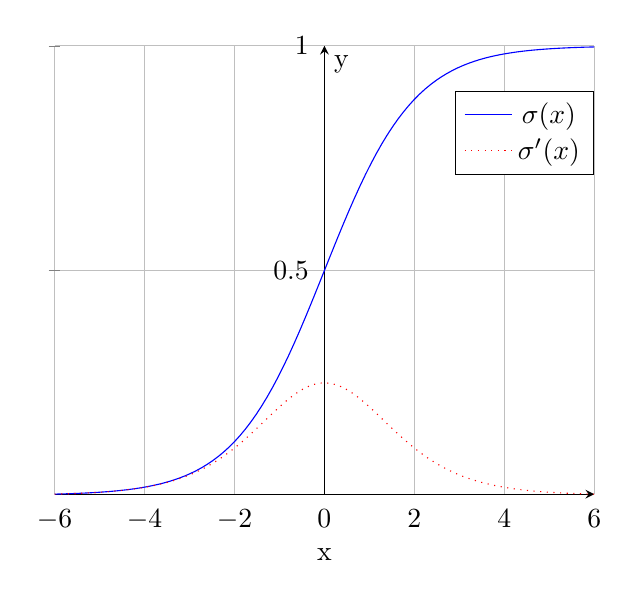
\begin{tikzpicture}[declare function={sigma(\x)=1/(1+exp(-\x));
    sigmap(\x)=sigma(\x)*(1-sigma(\x));}]
    \begin{axis}%
    [
        grid=major,     
        xmin=-6,
        xmax=6,
        axis x line=bottom,
        ytick={0,.5,1},
        ymax=1,
        ylabel= y,
        xlabel= x,
        ytick align=outside,
        ytick pos=left,
        major x tick style = transparent,
        axis y line=middle,
        samples=100,
        domain=-6:6,
        legend style={at={(1,0.9)}}     
    ]
        \addplot[blue,mark=none]   (x,{sigma(x)});
        \addplot[red,dotted,mark=none]   (x,{sigmap(x)});
        \legend{$\sigma(x)$,$\sigma'(x)$}
    \end{axis}
    \end{tikzpicture}
    
    \caption{Sigmoid function and its derivative.}
    \label{fig:sigmoid}
\end{figure}
\textbf{mer?}

\subsection{Neural network}
\begin{figure}[hp]
\centering
\def\layersep{2.5cm}
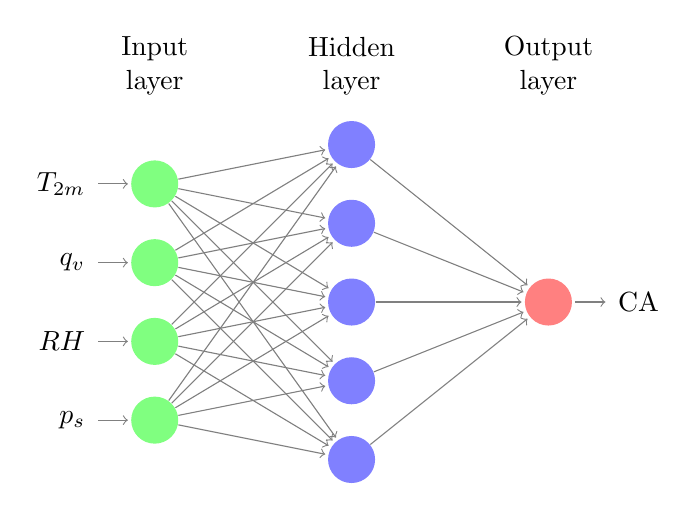
\begin{tikzpicture}[shorten >=1pt,->,draw=black!50, node distance=\layersep]
    \tikzstyle{every pin edge}=[<-,shorten <=1pt]
    \tikzstyle{neuron}=[circle,fill=black!25,minimum size=17pt,inner sep=0pt]
    \tikzstyle{input neuron}=[neuron, fill=green!50];
    \tikzstyle{output neuron}=[neuron, fill=red!50];
    \tikzstyle{hidden neuron}=[neuron, fill=blue!50];
    \tikzstyle{annot} = [text width=4em, text centered]

    \node[input neuron, pin=left:$T_{2m}$] (I-1) at (0,-1) {};
    \node[input neuron, pin=left:$q_v$] (I-2) at (0,-2) {};
    \node[input neuron, pin=left:$RH$] (I-3) at (0,-3) {};
    \node[input neuron, pin=left:$p_s$] (I-4) at (0,-4) {};

    % Draw the input layer nodes
    %\foreach \name / \y in {1,...,4}
    % This is the same as writing \foreach \name / \y in {1/1,2/2,3/3,4/4}
    %    \node[input neuron, pin=left:Input \#\y] (I-\name) at (0,-\y) {};

    % Draw the hidden layer nodes
    \foreach \name / \y in {1,...,5}
        \path[yshift=0.5cm]
            node[hidden neuron] (H-\name) at (\layersep,-\y cm) {};

    % Draw the output layer node
    \node[output neuron,pin={[pin edge={->}]right:CA}, right of=H-3] (O) {};

    % Connect every node in the input layer with every node in the
    % hidden layer.
    \foreach \source in {1,...,4}
        \foreach \dest in {1,...,5}
            \path (I-\source) edge (H-\dest);

    % Connect every node in the hidden layer with the output layer
    \foreach \source in {1,...,5}
        \path (H-\source) edge (O);

    % Annotate the layers
    \node[annot,above of=H-1, node distance=1cm] (hl) {Hidden layer};
    \node[annot,left of=hl] {Input layer};
    \node[annot,right of=hl] {Output layer};
\end{tikzpicture}

\caption{One layer hidden neural network. Taking temperature, humidities and pressure as input and estimating a fractional cloud cover - cloud amount - CA}
\label{fig:one_layer_mlp}
\end{figure}
Figure \ref{fig:one_layer_mlp} shows a simple architecture of a neural network. This consist of four input nodes or neurons, one for each of the variables relevant for the problem at hand. This is a fully connected network, meaning that every input node has a connection/weight to the next layer. After the input data has been passed to the hidden layer (sum over the matrix multiplication of the data and weight) it goes though a activation. The activation function in neural networks introduce the non-linearity's. Without then this would be piece-wise linear functions\textbf{..?}. Figure \ref{fig:activation_one_node} illustrates the activation in one node based on the input of variables. 
\begin{figure}[hp]
\centering
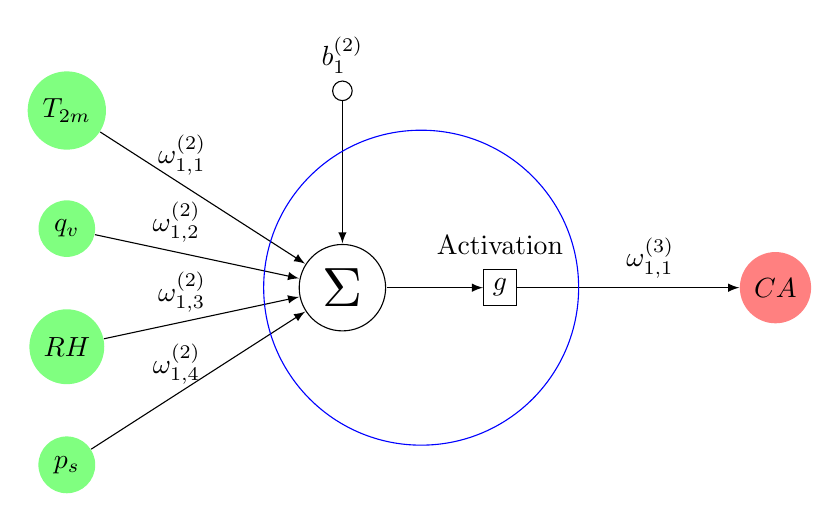
\begin{tikzpicture}[>=latex]
\path
(0,0)     node[circle,draw,scale=2,inner sep=2pt] (S) {$\Sigma$}
+(90:2.5) node[circle,draw,inner sep=2.5pt] (b) {}
          node[above=1mm] {$b_1^{(2)}$}
+(-3.5,2.25)  node[circle,fill=green!50]  (x1) {$T_{2m}$}
+(-3.5,0.75)    node[circle,fill=green!50]  (x2) {$q_v$}
+(-3.5,-0.75) node[circle,fill=green!50]  (x3) {$RH$}
+(-3.5,-2.25) node[circle,fill=green!50]  (x4) {$p_s$}
(2,0)    node[draw] (g) {$g$} node[above=3mm]{Activation}
+(3.5,0)  node[circle,fill=red!50]  (y1) {$CA$};
%+(-15:3) node[circle,fill=red!50]  (y2) {$\hat{y}_2$};
\draw[->] (S)--(g);
\draw[->] (b)--(S);
\draw[->] (g)--(y1) node[pos=.6,above]{$\omega_{1,1}^{(3)}$};
%\draw[->] (g)--(y2) node[pos=.6,below]{$\omega_{2,1}^{(3)}$};
\draw[->] (x1)--(S) node[pos=.4,above]{$\omega_{1,1}^{(2)}$};
\draw[->] (x2)--(S) node[pos=.4,above]{$\omega_{1,2}^{(2)}$};
\draw[->] (x3)--(S) node[pos=.4,above]{$\omega_{1,3}^{(2)}$};
\draw[->] (x4)--(S) node[pos=.4,above]{$\omega_{1,4}^{(2)}$};
\draw[blue] (1,0) circle(2);
\end{tikzpicture}

\caption{Sketch of the activation on one of the nodes in the hidden layer. Edit figure to have one output node. Consider using another subscript than g for activation function..?}
\label{fig:activation_one_node}
\end{figure}
In a neural network the connections between the nodes and the biases of the nodes need to be trained. This means that the optimal first layer in three layer model, is not equal to the optimal first layer in a two layer model. 
\\ \\
Three important concepts to every model. The weights, loss-function and optimiser. \textbf{neurons..?} The models is built from weights. The loss is a measure on how close you are to what you want to learn. Optimiser updates/adjust the weights in the direction of a lower loss. \textbf{Backpropagation is the learning algorithmn?} 
\begin{equation} \label{eq:relating_cc_as_a_func}
    tcc = f(T_{2m}, q_v, RH, sp)
\end{equation}
The rules I hope to achieve in this thesis is the physical relation of total cloud cover based on temperature, pressure and humidity. Like described in equation  \eqref{eq:relating_cc_as_a_func}.

Explain Difference between a neural network used for classification and regression, is choises in cost-function and activation function in the output layer (linear for regression and softmax for classification). 

\subsection{Recurrent networks}
Introduction to recurrent networks. 

\subsubsection{Convolution}
Convolution is a mathematical operation where you move a filter across you two dimensional data. Here the result in one cell is the affected by its neighbours. In a convolution neural network the trained weights are the filters. 
% kilde https://tex.stackexchange.com/questions/522118/visualizing-matrix-convolution 
\begin{figure}[hp]
    \centering
    \begin{tikzpicture}[mmat/.style={matrix of math nodes,column sep=-\pgflinewidth/2,
   row sep=-\pgflinewidth/2,cells={nodes={draw,inner sep=2pt,thin}},draw=#1,thick,inner sep=0pt},
   mmat/.default=black,
   node distance=0.3em]
 \matrix[mmat](mat1){
         0 & 1 & 1 & 1 & 0 & 0 & 0 \\ 
         0 & 0 & 1 & 1 & 1 & 0 & 0 \\ 
         0 & 0 & 0 & 1 & 1 & 1 & 0 \\ 
         0 & 0 & 0 & 1 & 1 & 0 & 0 \\ 
         0 & 0 & 1 & 1 & 0 & 0 & 0 \\ 
         0 & 1 & 1 & 0 & 0 & 0 & 0 \\ 
         0 & 1 & 0 & 0 & 0 & 0 & 0 \\ 
         };
 \node[fit=(mat1-1-4)(mat1-3-6),inner sep=0pt,draw,red,thick](f1){};        
 \node[right=of mat1] (mul) {$*$};      
 \matrix[mmat=blue,fill=blue!20,right=of mul](mat2){    
     1 & 0 & 1 \\ 
     0 & 1 & 0 \\ 
     1 & 0 & 1 \\ };
 \node[right=of mat2] (eq) {$=$};       
 \matrix[mmat,right=of eq](mat3){    
     1 & 4 & 3 & |[draw=green,thick,fill=green!20,alias=4]|4 & 1 \\ 
     1 & 2 & 4 & 3 & 3 \\ 
     1 & 2 & 3 & 4 & 1 \\ 
     1 & 3 & 3 & 1 & 1 \\ 
     3 & 3 & 1 & 1 & 0 \\ 
 };
 \foreach \Anchor in {south west,north west,south east,north east}
 {\draw[blue,densely dotted] (f1.\Anchor) -- (mat2.\Anchor); 
 \draw[green,densely dotted] (4.\Anchor) -- (mat2.\Anchor);}
 \begin{scope}[on background layer]
  \fill[red!20] (f1.north west) rectangle (f1.south east);
 \end{scope}
\end{tikzpicture}
    \caption{Diagram showing a convolutional operation.}
    \label{fig:convolution}
\end{figure}

% By J. Leon, Beerware licence is acceptable...
% https://tex.stackexchange.com/questions/432312/how-do-i-draw-an-lstm-cell-in-tikz?rq=1

% used to avoid putting the same thing several times...
% Command \empt{var1}{var2}
\newcommand{\empt}[2]{$#1^{\langle #2 \rangle}$}
\begin{figure}[hp]
    \centering
    
    \begin{tikzpicture}[
    % GLOBAL CFG
    font=\sf \scriptsize,
    >=LaTeX,
    % Styles
    cell/.style={% For the main box
        rectangle, 
        rounded corners=5mm, 
        draw,
        very thick,
        },
    operator/.style={%For operators like +  and  x
        circle,
        draw,
        inner sep=-0.5pt,
        minimum height =.2cm,
        },
    function/.style={%For functions
        ellipse,
        draw,
        inner sep=1pt
        },
    ct/.style={% For external inputs and outputs
        circle,
        draw,
        line width = .75pt,
        minimum width=1cm,
        inner sep=1pt,
        },
    gt/.style={% For internal inputs
        rectangle,
        draw,
        minimum width=4mm,
        minimum height=3mm,
        inner sep=1pt
        },
    mylabel/.style={% something new that I have learned
        font=\scriptsize\sffamily
        },
    ArrowC1/.style={% Arrows with rounded corners
        rounded corners=.25cm,
        thick,
        },
    ArrowC2/.style={% Arrows with big rounded corners
        rounded corners=.5cm,
        thick,
        },
    ]

%Start drawing the thing...    
    % Draw the cell: 
    \node [cell, minimum height =4cm, minimum width=6cm, fill = green
    , opacity=0.2] at (0,0){} ;

    % Draw inputs named ibox#
    \node [gt, fill = yellow] (ibox1) at (-2,-0.75) {$\sigma$};
    \node [gt, fill = yellow] (ibox2) at (-1.5,-0.75) {$\sigma$};
    \node [gt, minimum width=1cm, fill = yellow] (ibox3) at (-0.5,-0.75) {Tanh};
    \node [gt, fill = yellow] (ibox4) at (0.5,-0.75) {$\sigma$};

   % Draw opérators   named mux# , add# and func#
    \node [operator, fill = pink] (mux1) at (-2,1.5) {$\times$};
    \node [operator, fill = pink] (add1) at (-0.5,1.5) {+};
    \node [operator, fill = pink] (mux2) at (-0.5,0) {$\times$};
    \node [operator, fill = pink] (mux3) at (1.5,0) {$\times$};
    \node [function, fill = pink] (func1) at (1.5,0.75) {Tanh};

    % Draw External inputs? named as basis c,h,x
    \node[ct, label={[mylabel]Cell state}] (c) at (-4,1.5) {\empt{c}{t-1}};
    \node[ct, label={[mylabel]Hidden state}, fill = purple, opacity =0.3] (h) at (-4,-1.5) {\empt{h}{t-1}};
    \node[ct, label={[mylabel]left:Input}, fill = blue, opacity =0.3] (x) at (-2.5,-3) {\empt{x}{t}};

    % Draw External outputs? named as basis c2,h2,x2
    \node[ct, label={[mylabel]Cell state}] (c2) at (4,1.5) {\empt{c}{t}};
    \node[ct, label={[mylabel]Hidden state}, fill = purple, opacity =0.3] (h2) at (4,-1.5) {\empt{h}{t}};
    \node[ct, label={[mylabel]left:Output}, fill = purple, opacity =0.3] (x2) at (2.5,3) {\empt{h}{t}};
    
    % Start connecting all.
    
    % Intersections and displacements are used. 
    % Drawing arrows    
    \draw [ArrowC1] (c) -- (mux1) -- (add1) -- (c2);

    % Inputs
    \draw [ArrowC2] (h) -| (ibox4) ;
    \draw [ArrowC1] (h -| ibox1)++(-0.5,0) -| (ibox1); 
    \draw [ArrowC1] (h -| ibox2)++(-0.5,0) -| (ibox2);
    \draw [ArrowC1] (h -| ibox3)++(-0.5,0) -| (ibox3);
    \draw [ArrowC1] (x) -- (x |- h)-| (ibox3);

    % Internal - possibility , rotate = 90
    \draw [->, ArrowC2] (ibox1) -- (mux1) node[midway, left] {F};
    \draw [->, ArrowC2] (ibox2) |- (mux2) node[midway, above] {I};
    \draw [->, ArrowC2] (ibox3) -- (mux2) node[midway, right] {$\Tilde{C}$};
    \draw [->, ArrowC2] (ibox4) |- (mux3) ; %node[midway, above] {b};
    \draw [->, ArrowC2] (mux2) -- (add1) ; %node[midway, above] {c};
    \draw [->, ArrowC1] (add1 -| func1)++(-0.5,0) -| (func1) ; % node[midway, above] {d};
    \draw [->, ArrowC2] (func1) -- (mux3) node[midway, right] {O};

    %Outputs
    \draw [-, ArrowC2] (mux3) |- (h2);
    \draw (c2 -| x2) ++(0,-0.1) coordinate (i1);
    \draw [-, ArrowC2] (h2 -| x2)++(-0.5,0) -| (i1);
    \draw [-, ArrowC2] (i1)++(0,0.2) -- (x2);
    %\node [cell, minimum height =4cm, minimum width=6cm, fill = pink, opacity=.8] at (0,0){\Large A} ;
    
\end{tikzpicture}
    \caption{Architecture of a \acrshort{lstm} cell. https://tex.stackexchange.com/questions/328733/how-to-draw-recurrent-neural-network for drawing multiple cells RNN.}
    \label{fig:lstm_cell}
\end{figure}


\input{Chapter2_Theory/tikz/spherical_vs_cartesian.tikz}

\begin{figure}
    \centering
    \includegraphics{Chapter2_Theory/images/classification_overfitted.png}
    \caption{Caption}
    \label{fig:classification_overfitting}
\end{figure}

Climate models are implementations of physical equations and parametrizations. After some tuning they are thought to provide the answers given a state. You can read more about climate models in section \ref{sec:climate_models}. Since Hansen et. al. 1984 \textbf{siter} first attempted to estimate the \acrfull{ecs}, reaserchers have been working on reducing the spread. 
More complex models introduce other uncertainties and they have not yet been able to reduce it sufficiently \textbf{hvordan si "nok" - uten at et blir slemt}. With data available, more complex relations can be described. This requires deeper networks and the depth in deep learning refers to the number of layers. More complex models come with a higher risk of overfitting. \textbf{Kilde book Chollet}.

\subsection{Metrics}  \label{sec:metrics}
In order to acquire a certain skill you need a measure determining how close you are. 
Use the sum of square or abosolute values in order to not penalize point on the lower side of the line. Or not having to deal with negative distances. 
\begin{equation} \label{eq:mse}
    MSE(\hat{y},\hat{\tilde{y}}) = \frac{1}{n} \sum_{i=0}^{n-1}(y_i-\tilde{y}_i)^2
\end{equation} 

\begin{equation} \label{eq:ase}
    ASE(\hat{y},\hat{\tilde{y}}) =  \sum_{i=0}^{n-1}(y_i-\tilde{y}_i)^2
\end{equation} 

\begin{equation} \label{eq:r2}
    R^2(\hat{y}, \tilde{\hat{y}}) = 1 - \frac{\sum_{i=0}^{n - 1} (y_i - \tilde{y}_i)^2}{\sum_{i=0}^{n - 1} (y_i - \bar{y})^2}
\end{equation} 
where mean value of $\hat{y}$ is defined as $\bar{y} =  \frac{1}{n} \sum_{i=0}^{n - 1} y_i$. $R^2$ describes how much of the variation in the dataset you are able to capture with your model.



\subsection{Hyperparameters - Automatic Optimization}
Keras-tuner.
\textbf{Explain all the params you tune. Might be beneficially with a figure. See Rune's MS-thesis.}



\subsubsection{Convolutional Neural Networks}
\input{Chapter2_Theory/tikz/cnn.tikz}


\subsubsection{Convolutional LSTM}
\label{sec:conv_lstm}
Key equations in convolutional LSTM is listed in equation (\ref{eq:CLSTM1_input_gate}) - (\ref{eq:CLSTM5_hidden_state}). Here $\circ$ denoted the Hademand product, which is a component wise multiplication, and * is convolution. 

\begin{equation} \label{eq:CLSTM1_input_gate}
    i_t = \sigma \left( W_{xi}*x_t + W_{hi}*H_{t-1} + W_{ci}\circ C_{t-1}+b_i \right) 
\end{equation}

\begin{equation} \label{eq:CLSTM2_forget_gate}
        f_t = \sigma \left( W_{xf}*x_t + W_{hf}*H_{t-1} + W_{cf}\circ C_{t-1}+b_f \right) 
\end{equation}

\begin{equation} \label{eq:CLSTM3_cellstate}
        C_t = f_t \circ C_{t-1} +i_t\circ tanh\left( W_{xc}*X_t + W_{hc}*H_{t-1} + b_c \right)
\end{equation}

\begin{equation} \label{eq:CLSTM4_output_gate}
        o_t = \sigma \left( W_{xo}*X_t + W_{ho}*H_{t-1} + W_{co}\circ C_{t}+b_o \right)
\end{equation}

\begin{equation} \label{eq:CLSTM5_hidden_state}
        H_t = o_t \circ tanh \left( C_t \right)
\end{equation}

\paragraph{Learning algorithmns - optimizen (implementation of sequence length)} \mbox{}\\
Describe the following
\begin{enumerate}
    \item Loss, cost, performance metric? epoch batch
\end{enumerate}

From Chollet book s. 11 \textit{the fundamental trick in deep learning is to use this score (result from performance metric) as a feedback signal to adjust the value of the weights a little, in a direction that will lower the loss score for the current example. } The adjustment is the job of the optimizer, which implements backpropagation algorithmn which is the sentral learning algoritmn.
\textbf{Explain this in words.}



\subsection{Klipp og lim}


When describing shapes, do it by keras convention. Which is channel first? \textbf{Talk about working with real data and not synthetic.} In this 
\textit{Learning means finding a suitable representation of model parameters that minimize a loss function for a given set of training data samples and their corresponding targets.}
\textbf{Does the setup here resemble videos mostly? Since its a sequence of frames containing meteorological data..}

\section{Future work}
\begin{enumerate}
    \item Describe how to make parametrization to implement in CMIP6.
    \item Programming language in climate models vs python.
\end{enumerate}






